\subsection{Aclaraciones de sintaxis}

Para mayor claridad y simpleza de las FSM, decidimos utilizar un abuso de notaci\'on para evitar escribir multiples transiciones.

\begin{figure}[H]
	\centering
	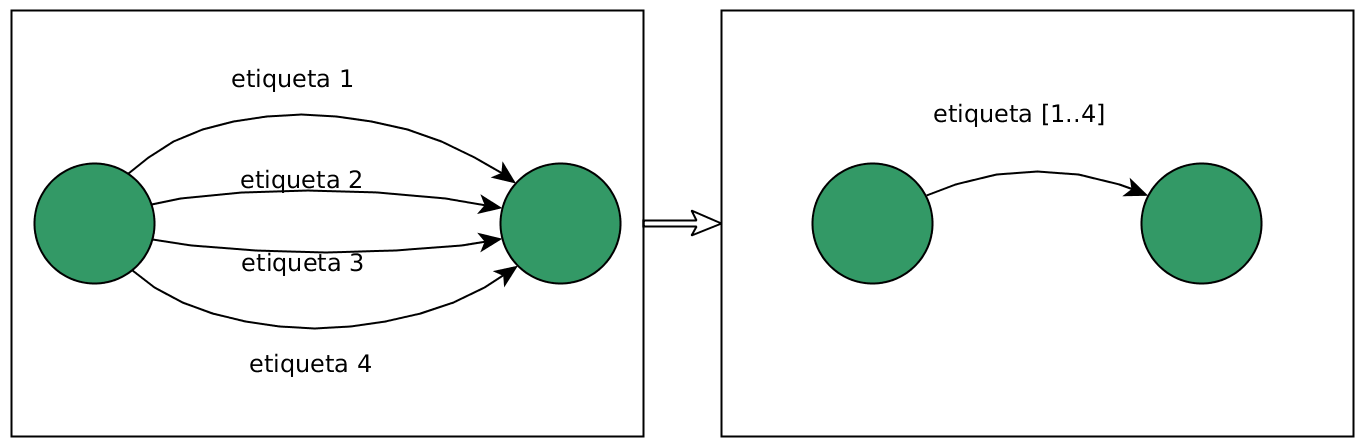
\includegraphics[scale=0.35]{imgs/fsm_ej1.png}
	\caption{Las transiciones numeradas con mismo nombre fueron reemplazadas por una \'unica transici\'on.}
\end{figure}

\begin{figure}[H]
	\centering
	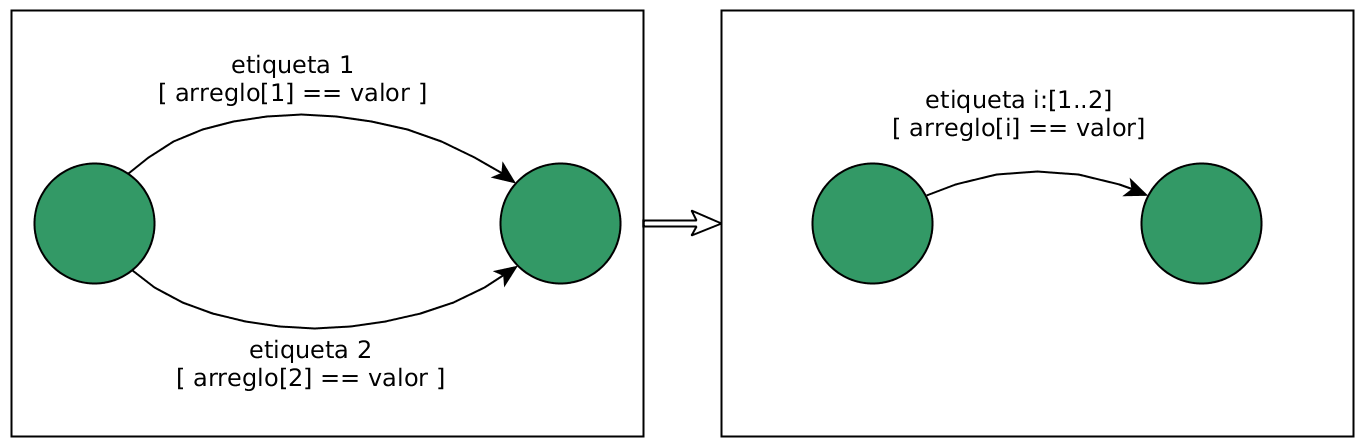
\includegraphics[scale=0.35]{imgs/fsm_ej2.png}
	\caption{Si en alg\'un momento deb\'iamos predicar sobre los n\'umeros en las etiquetas, le agregamos un iterador a la secuencia.}
\end{figure}

\subsection{Constantes y variables}

Constantes:
\begin{itemize}
\item CANT\_STOCK\_MAX es la cantidad máxima de stock en una estación. 
\item N es la cantidad de estaciones
\item M es la cantidad de habitantes en la ciudad
\item P es la cantidad total de empleados
\item ESTACION es un arreglo de P posiciones, donde ESTACION[e] es el número de la estación donde trabaja el empleado e.
\end{itemize}

Variables:
\begin{itemize}
\item stock[1..N]: [0..CANT\_STOCK\_MAX]
dasdasd
\item dondeEsta[1..M]: [0..N]. Indica, para cada usuario, en que estaci\'on se encuentra (si no se encuentra en ninguna estaci\'on el valor es 0).
\item pedido[1..N]: [-CANT\_STOCK\_MAX..CANT\_STOCK\_MAX]. Indica la cantidad de bicicletas que son enviadas a una estaci\'on. Si es para hacer un retiro de bicicletas el n\'umero es negativo. Una vez que el pedido llega o se va de la estaci\'on, el valor pasa a ser 0.
\item llegoPedido[1..N]: [0..1]. Cuando se recibe un pedido en una estaci\'on se pone el valor en 1, sino es 0.
\item atendidoPor[1..M]: [0..P]. Indica, para cada usuario, cu\'al es el empleado que lo est\'a atendiendo. Si a\'un no fue atendido, el valor es 0.
\end{itemize}

\subsection{FSM Sistema}

\begin{figure}[H]
	\centering
	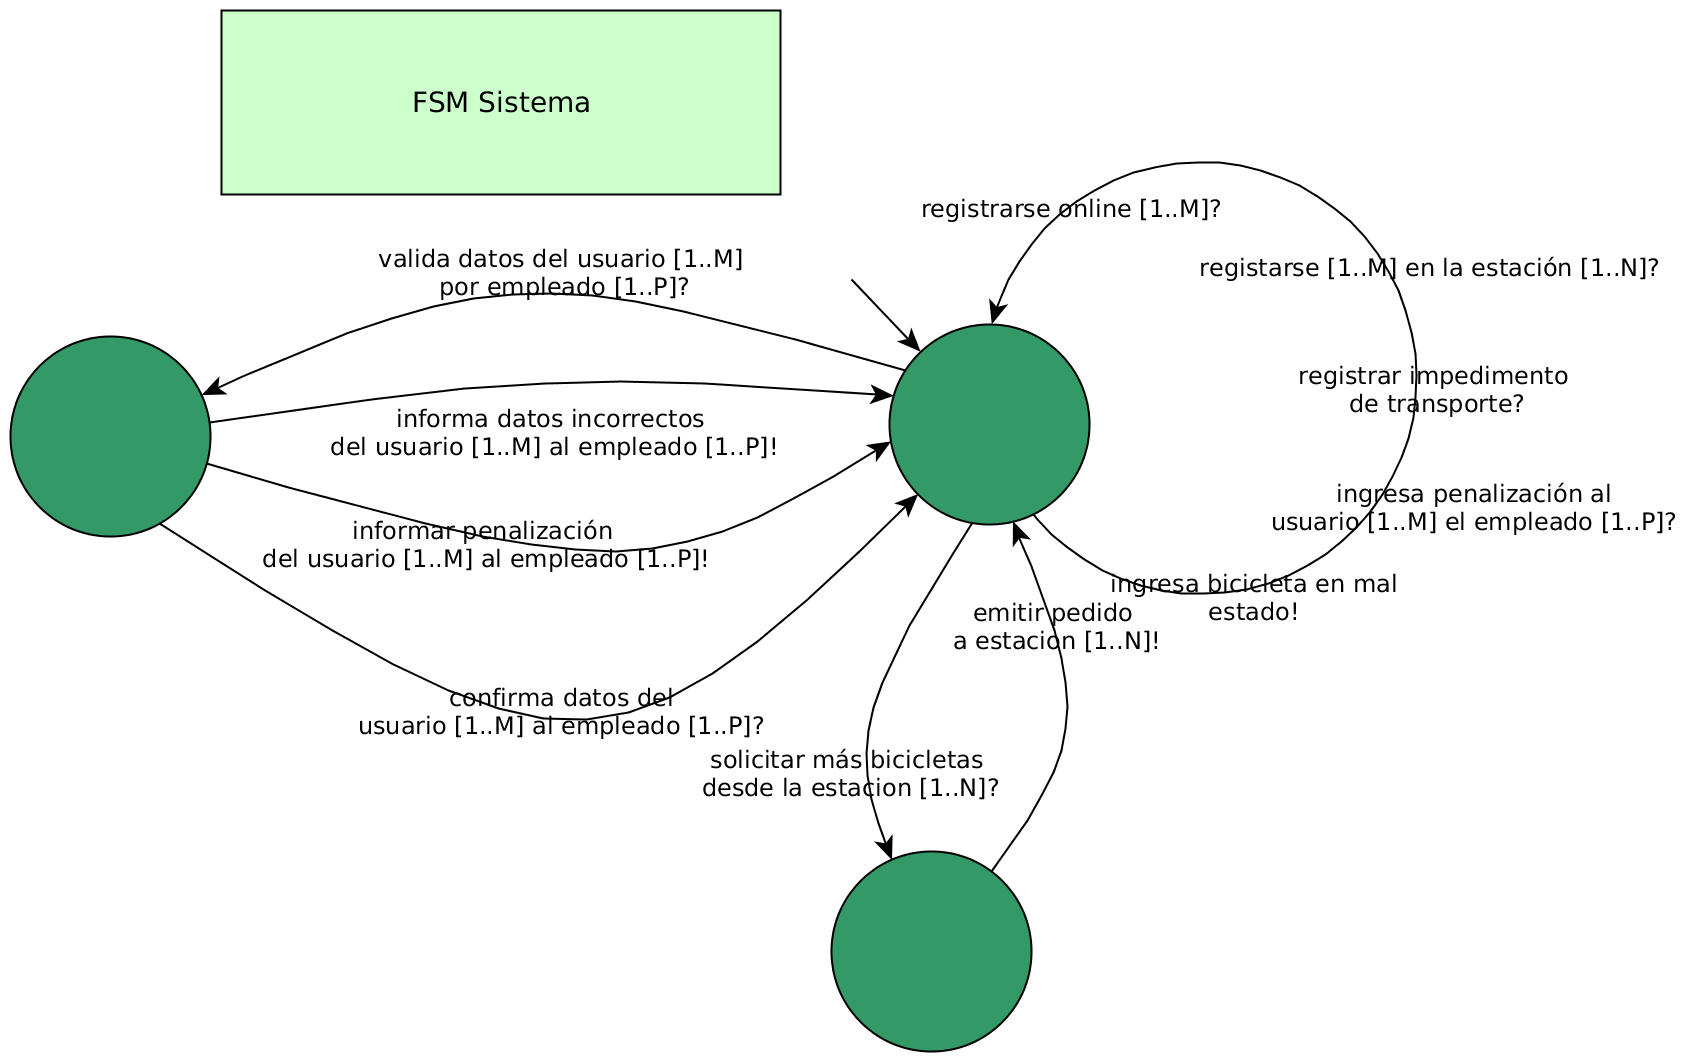
\includegraphics[scale=0.3]{imgs/fsm_sistema.png}
	\caption{FSM Sistema}
\end{figure}

\subsection{FSM Empresa de transporte}

\begin{figure}[H]
	\centering
	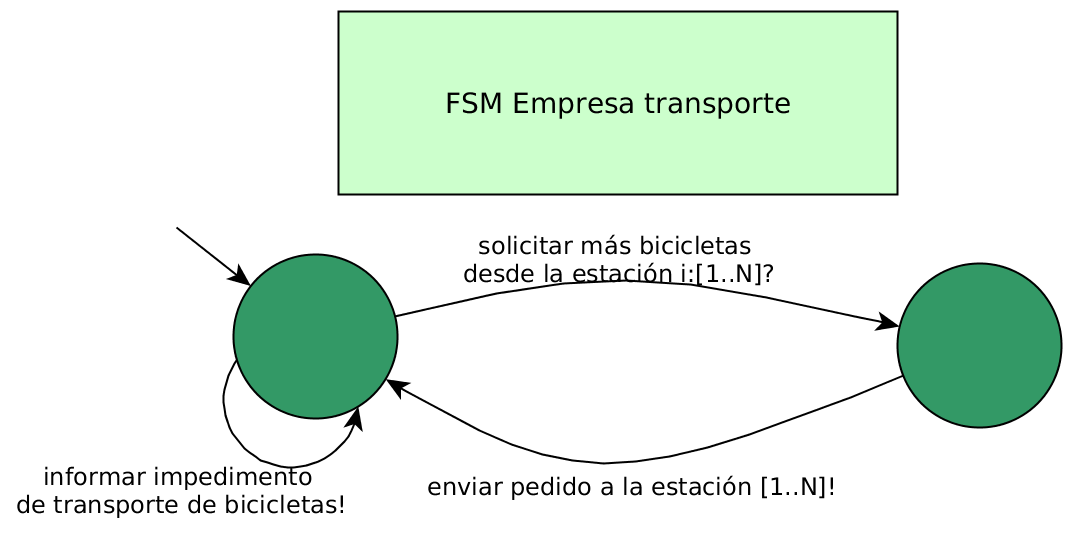
\includegraphics[scale=0.4]{imgs/fsm_empresa_transporte.png}
	\caption{FSM Empresa de transporte}
\end{figure}

\subsection{FSM Estaci\'on}

\begin{figure}[H]
	\centering
	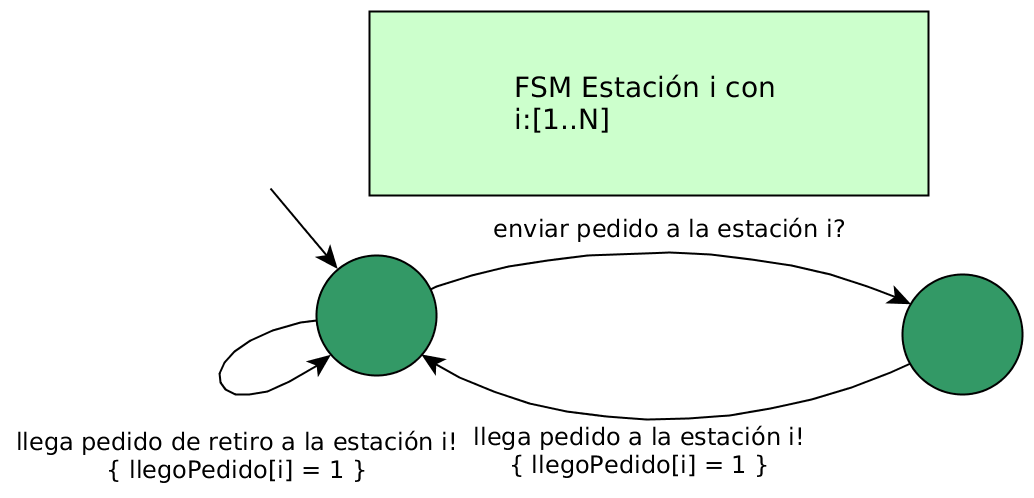
\includegraphics[scale=0.5]{imgs/fsm_estacion.png}
	\caption{FSM Estaci\'on}
\end{figure}

\subsection{FSM Controlador de stock}

\begin{figure}[H]
	\centering
	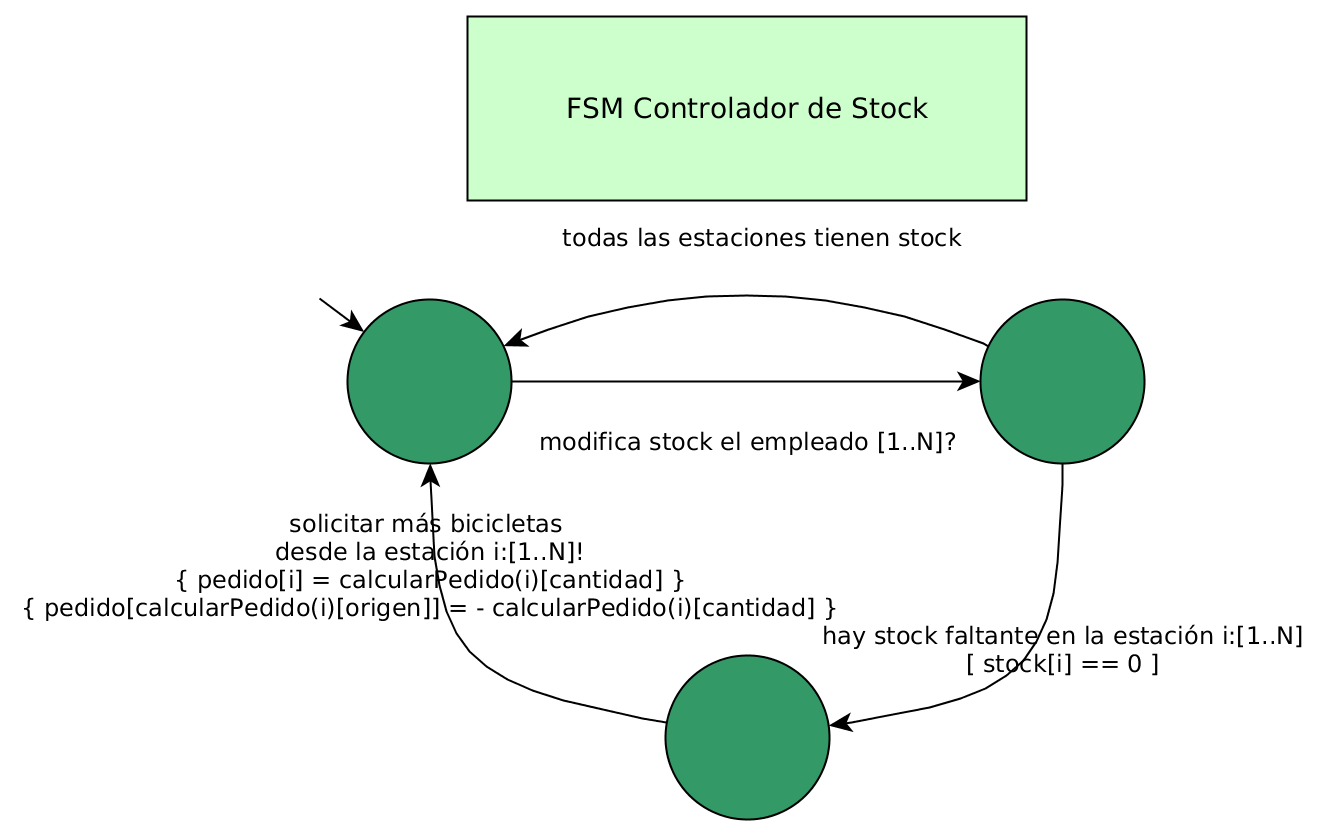
\includegraphics[scale=0.4]{imgs/fsm_controlador_stock.png}
	\caption{FSM Controlador de stock. \emph{calcularPedido(i)} es una funci\'on interna del sistema que calcula la cantidad de bicicletas a enviar\emph{([cantidad])} y desde d\'onde traerlas\emph{([origen])}.}
\end{figure}

Esta m\'aquina es una funcionalidad particular del sistema que dedicimos seperar para exhibir su comportamiento. Cada vez que un empleado modifica el stock de su estaci\'on, el controlador de stock se encarga de ver si la estaci\'on no m\'as bicicletas disponibles. En caso de ser as\'i, le avisa al sistema de que debe emitir un pedido de bicicletas. 

\subsection{FSM Empleado de gobierno}

\begin{figure}[H]
	\centering
	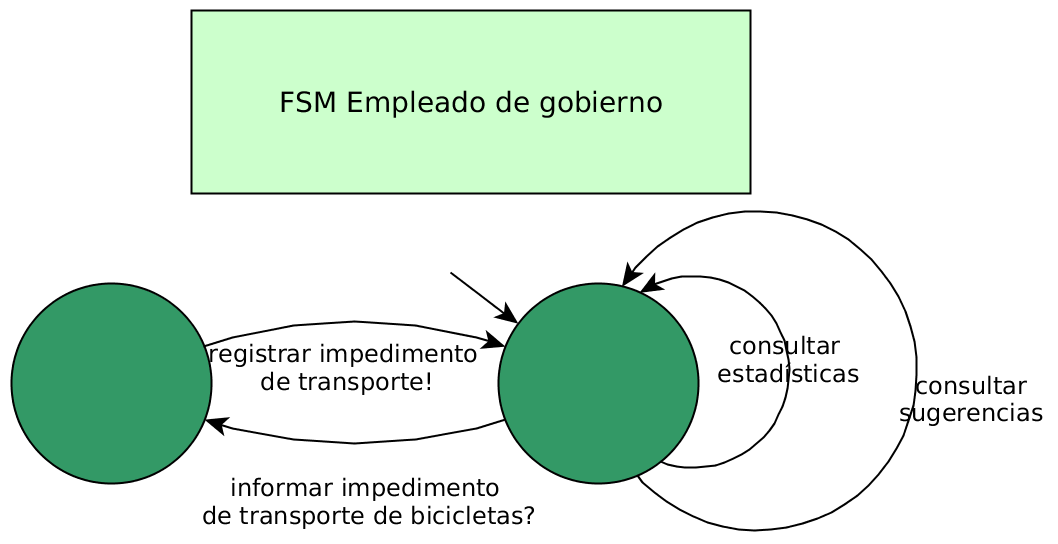
\includegraphics[scale=0.4]{imgs/fsm_empleado_gobierno.png}
	\caption{FSM Empleado de gobierno}
\end{figure}

\subsection{FSM Usuario}

\begin{figure}[H]
	\centering
	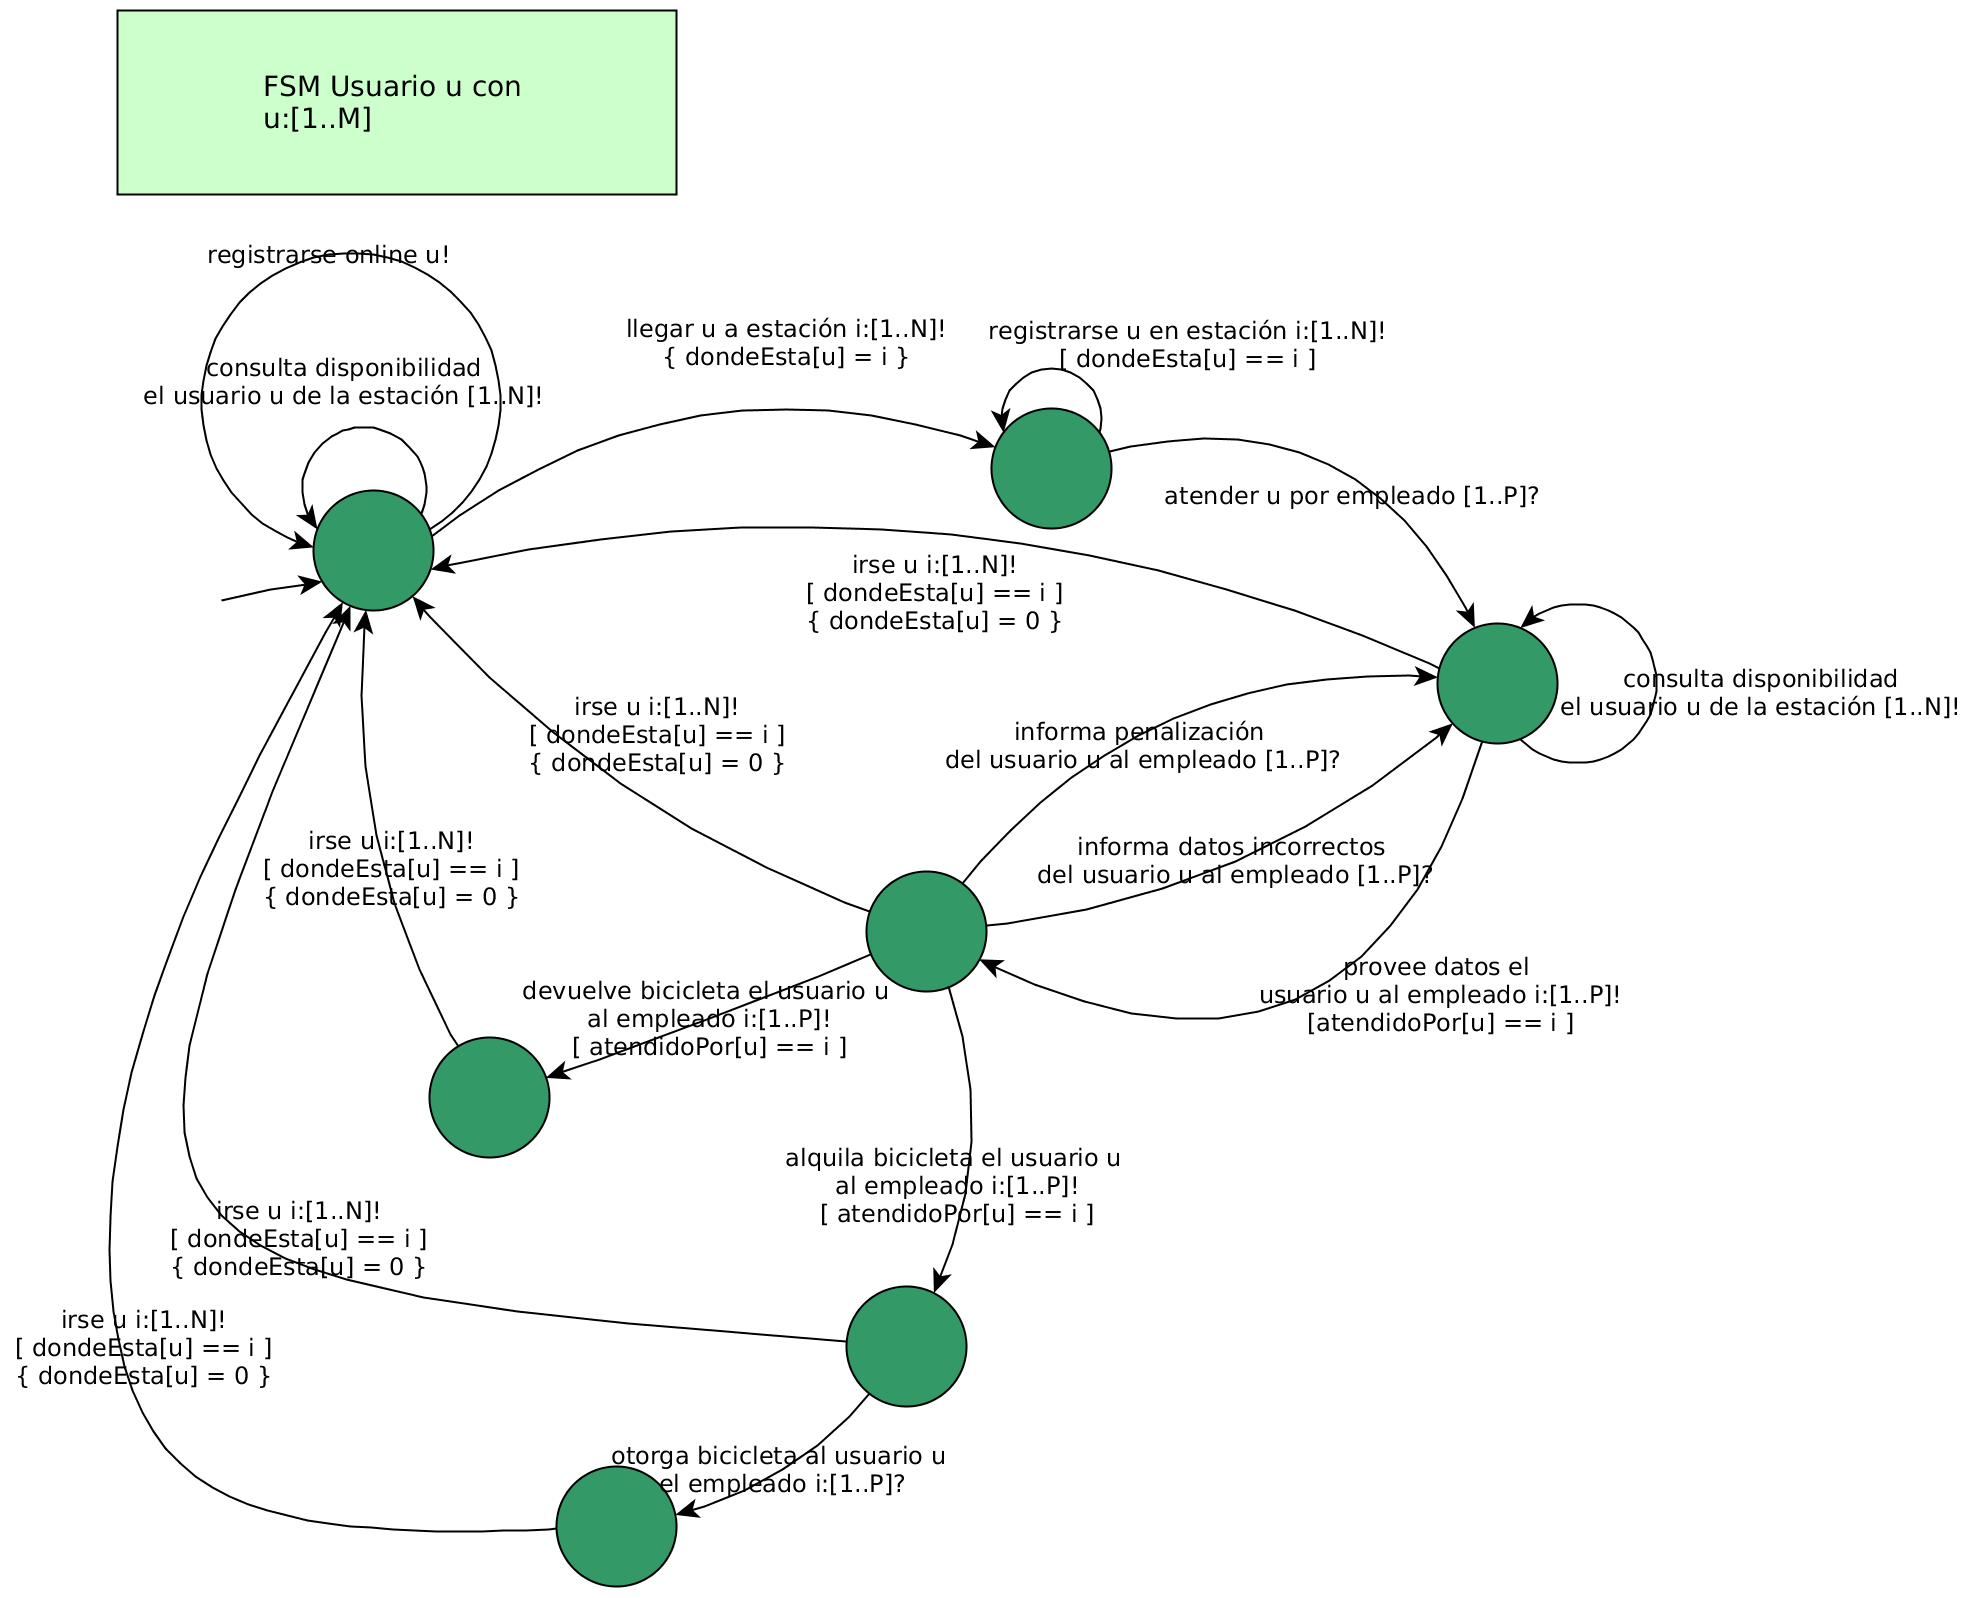
\includegraphics[scale=0.255]{imgs/fsm_usuario.png}
	\caption{FSM Usuario}
\end{figure}

\subsection{FSM Empleado}

\begin{figure}[H]
	\centering
	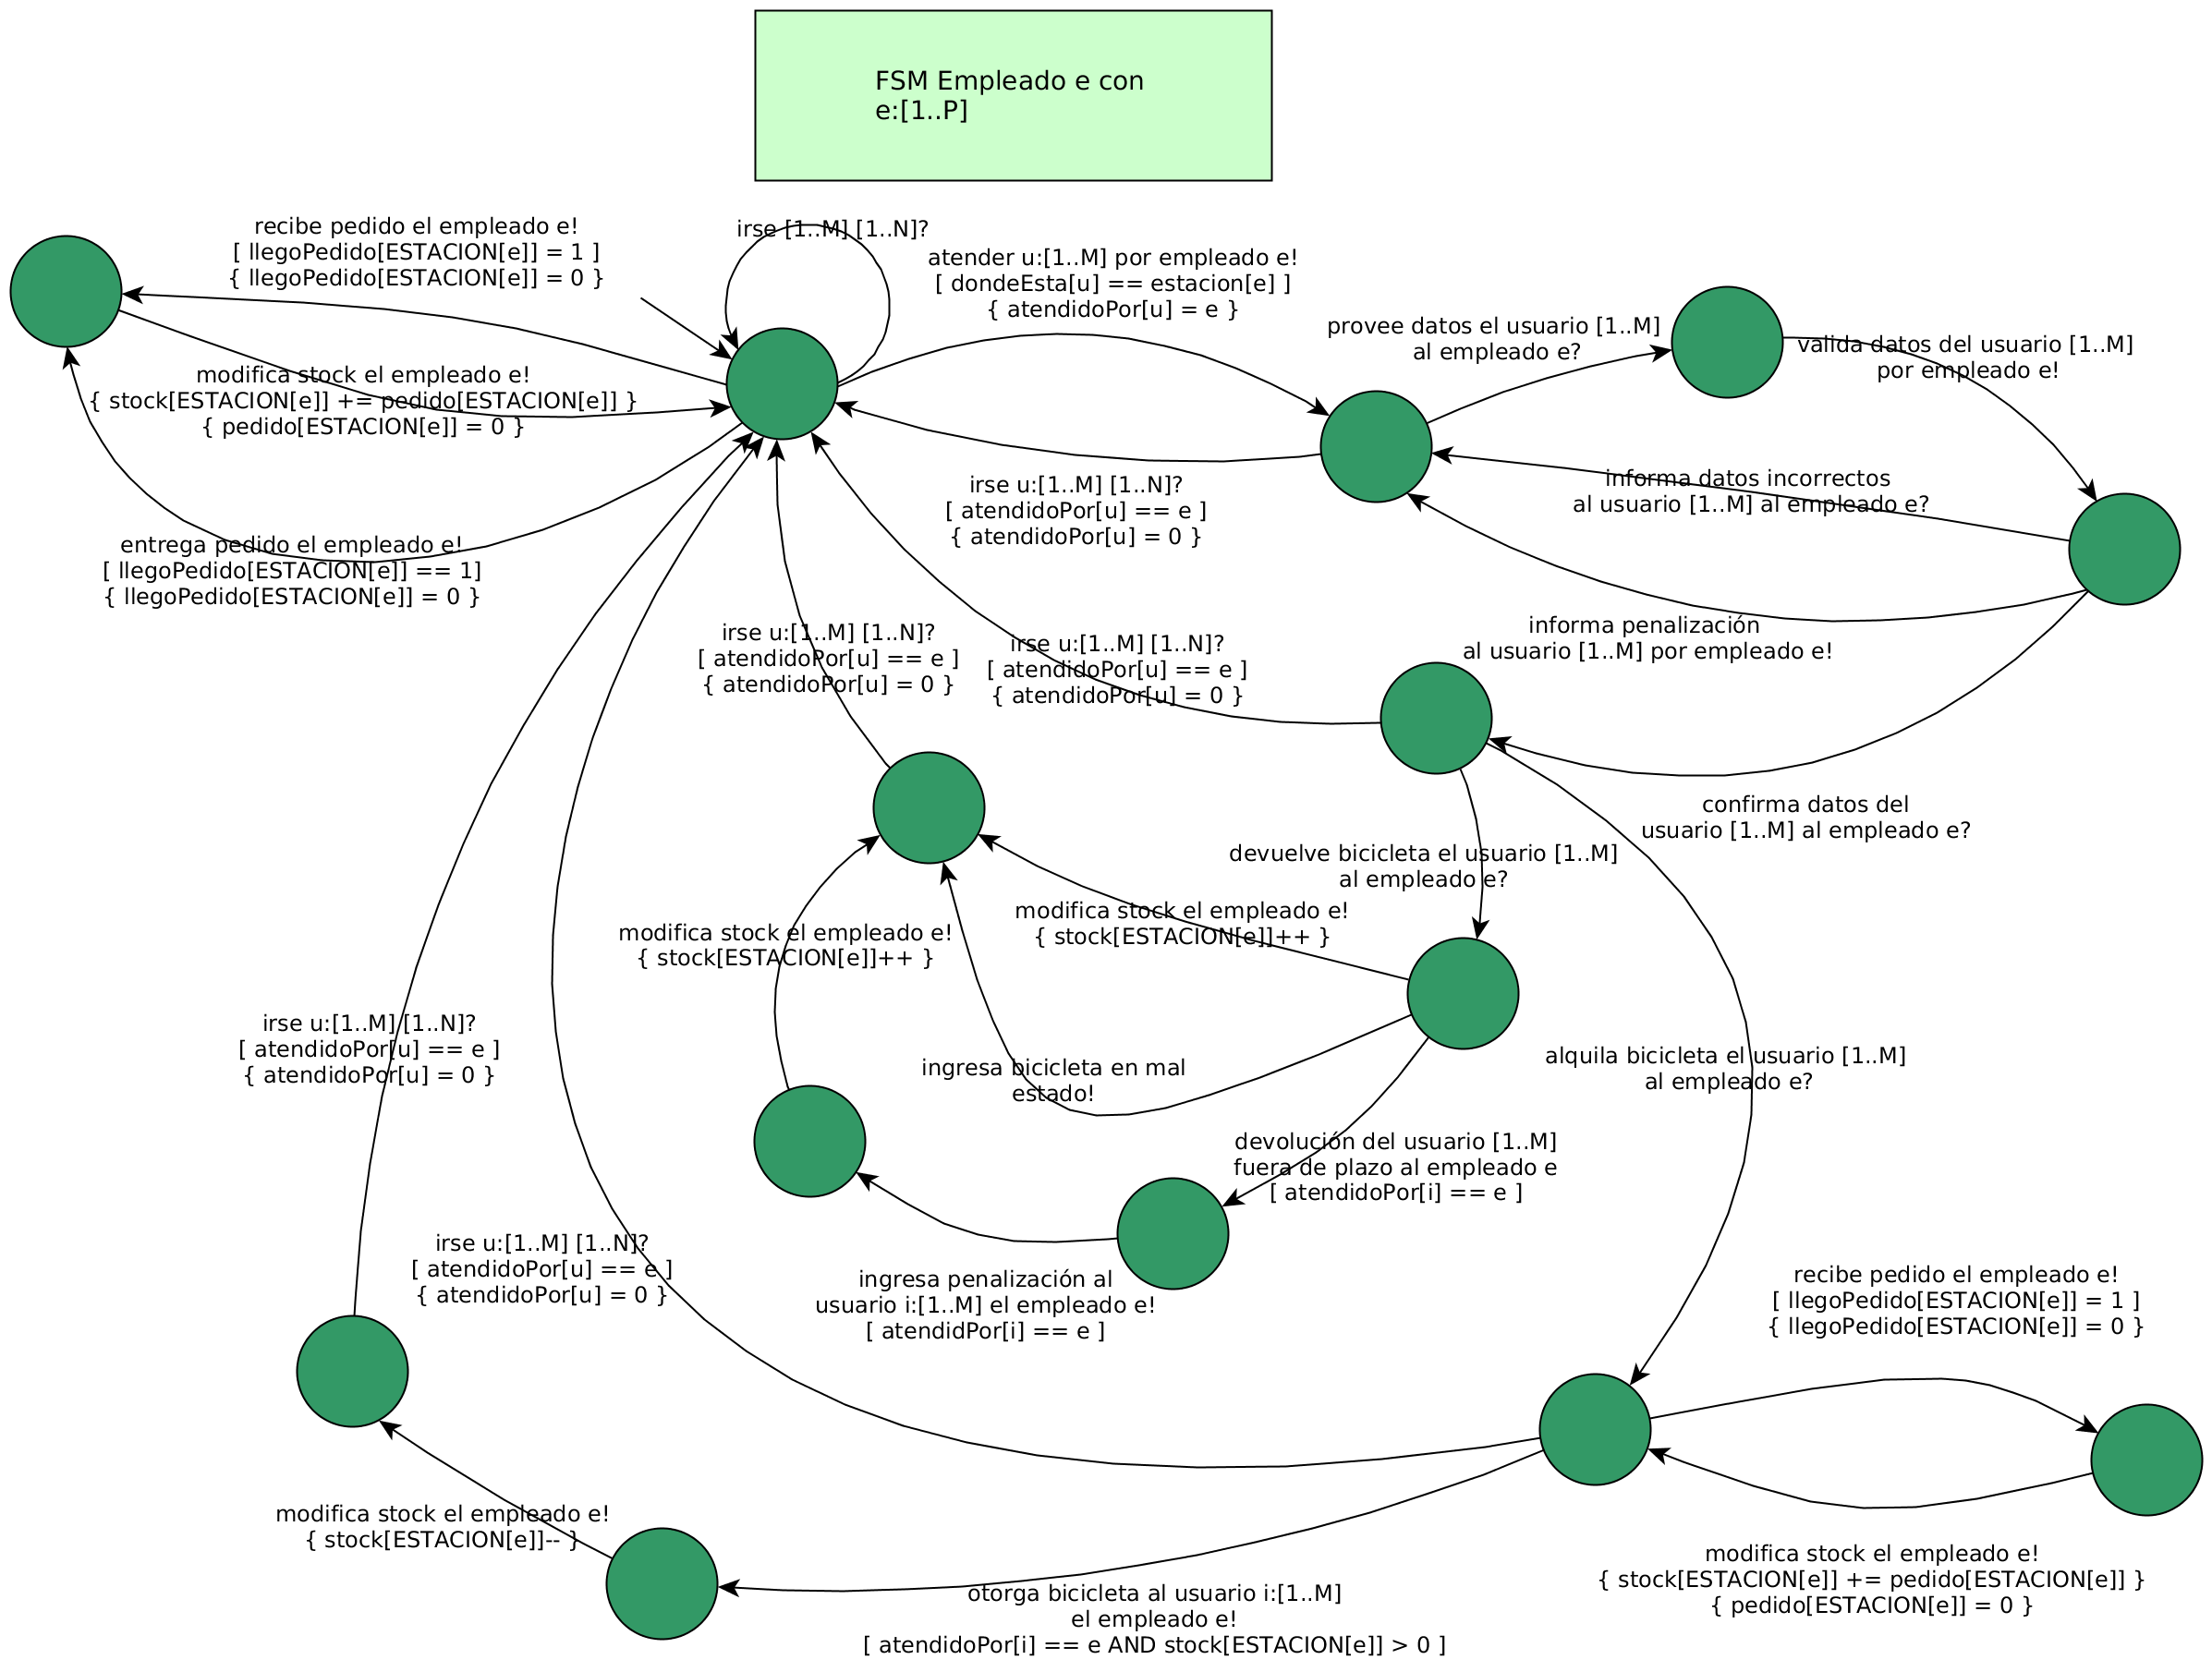
\includegraphics[scale=0.21]{imgs/fsm_empleado.png}
	\caption{FSM Empleado}
\end{figure}